%%%%%%%%%%%%%%%%%%%%%%%%%%%%%%%%%%%%%%%%%%%%%%%%%%%%%%%%%%%%%%%%%%%%%%%%%%%%%%%%%%%%%%%%%%%%%%%%%
% Cover slide
\frame[plain]{
\begin{center}
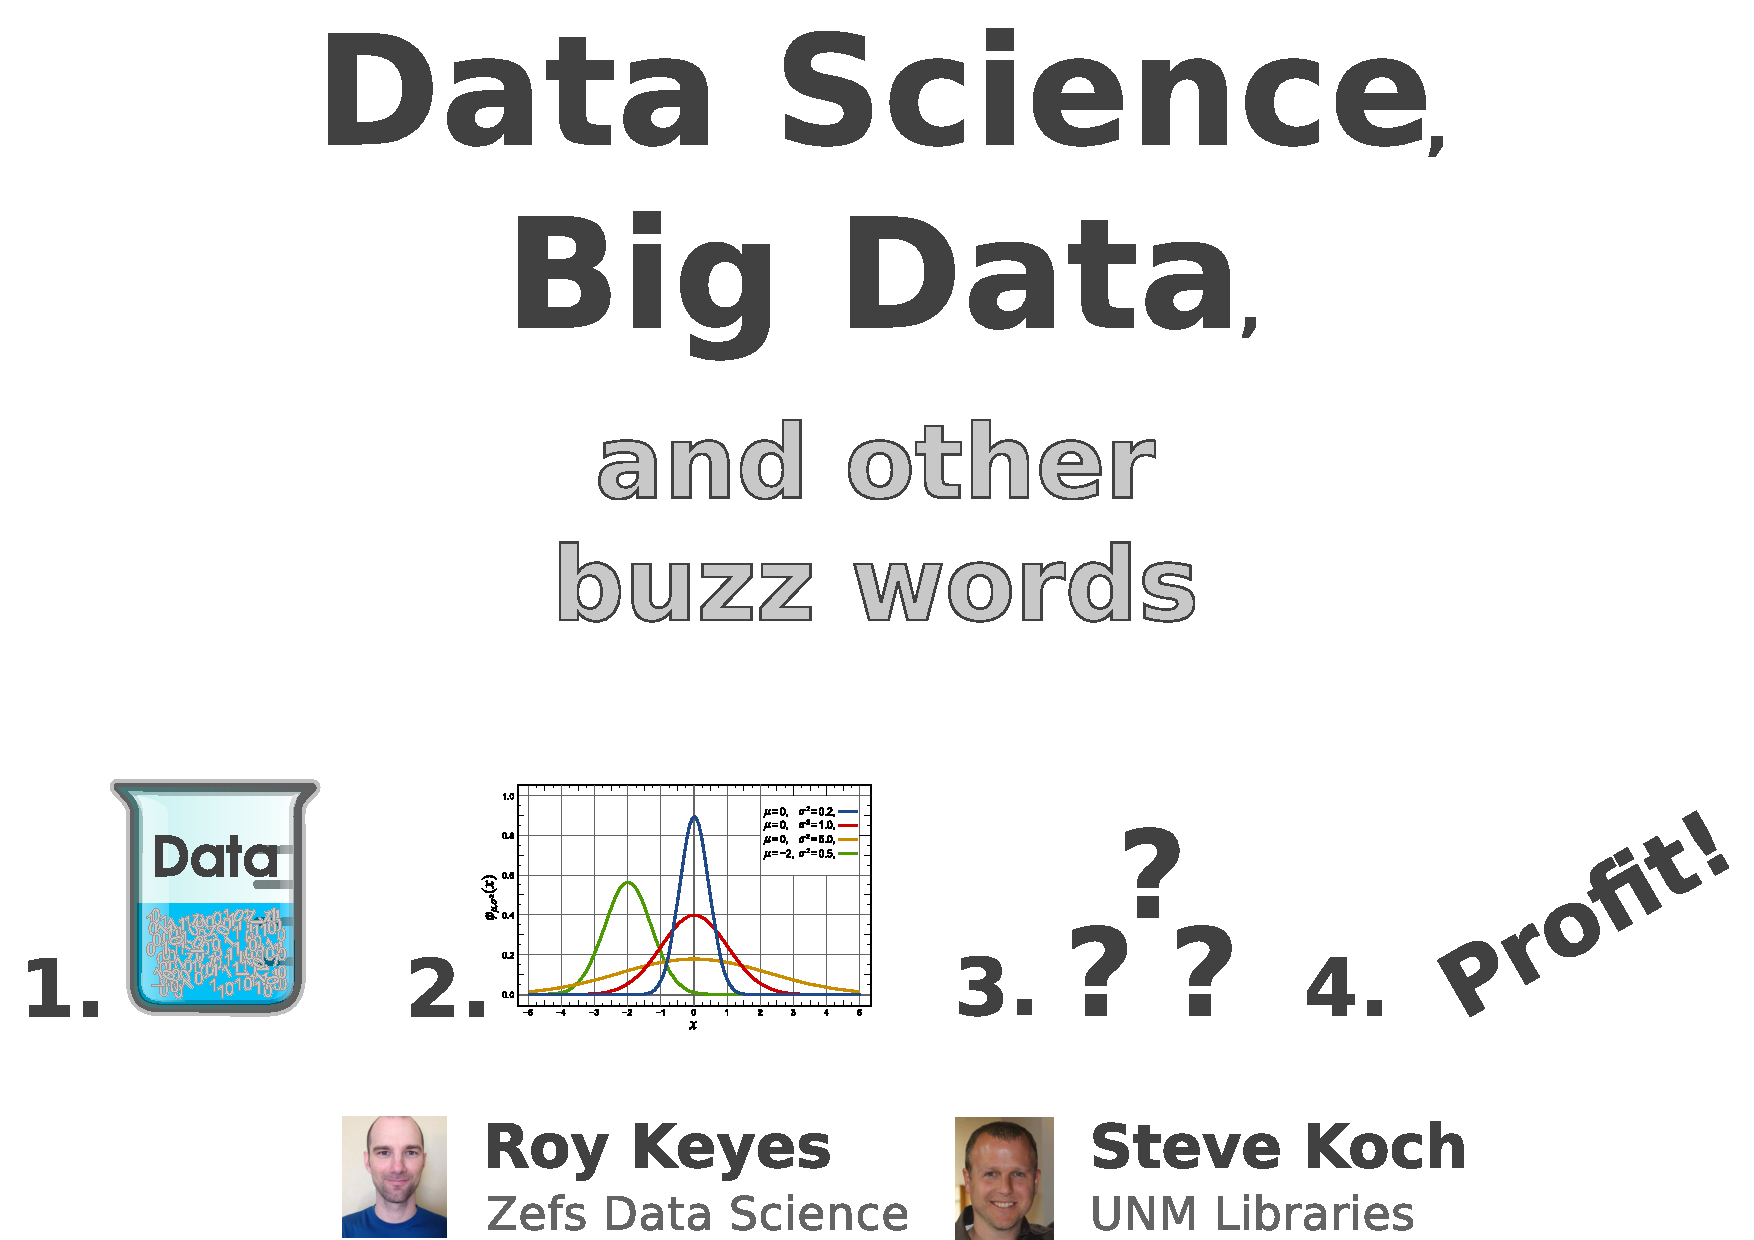
\includegraphics[width=1.0\textwidth]{graphics/data_title2.pdf}
\end{center}
}

%%%%%%%%%%%%%%%%%%%%%%%%%%%%%%%%%%%%%%%%%%%%%%%%%%%%%%%%%%%%%%%%%%%%%%%%%%%%%%%%%%%%%%%%%%%%%%%%%

\begin{frame}
%\frametitle{Suddenly data is everywhere!}
\begin{center}
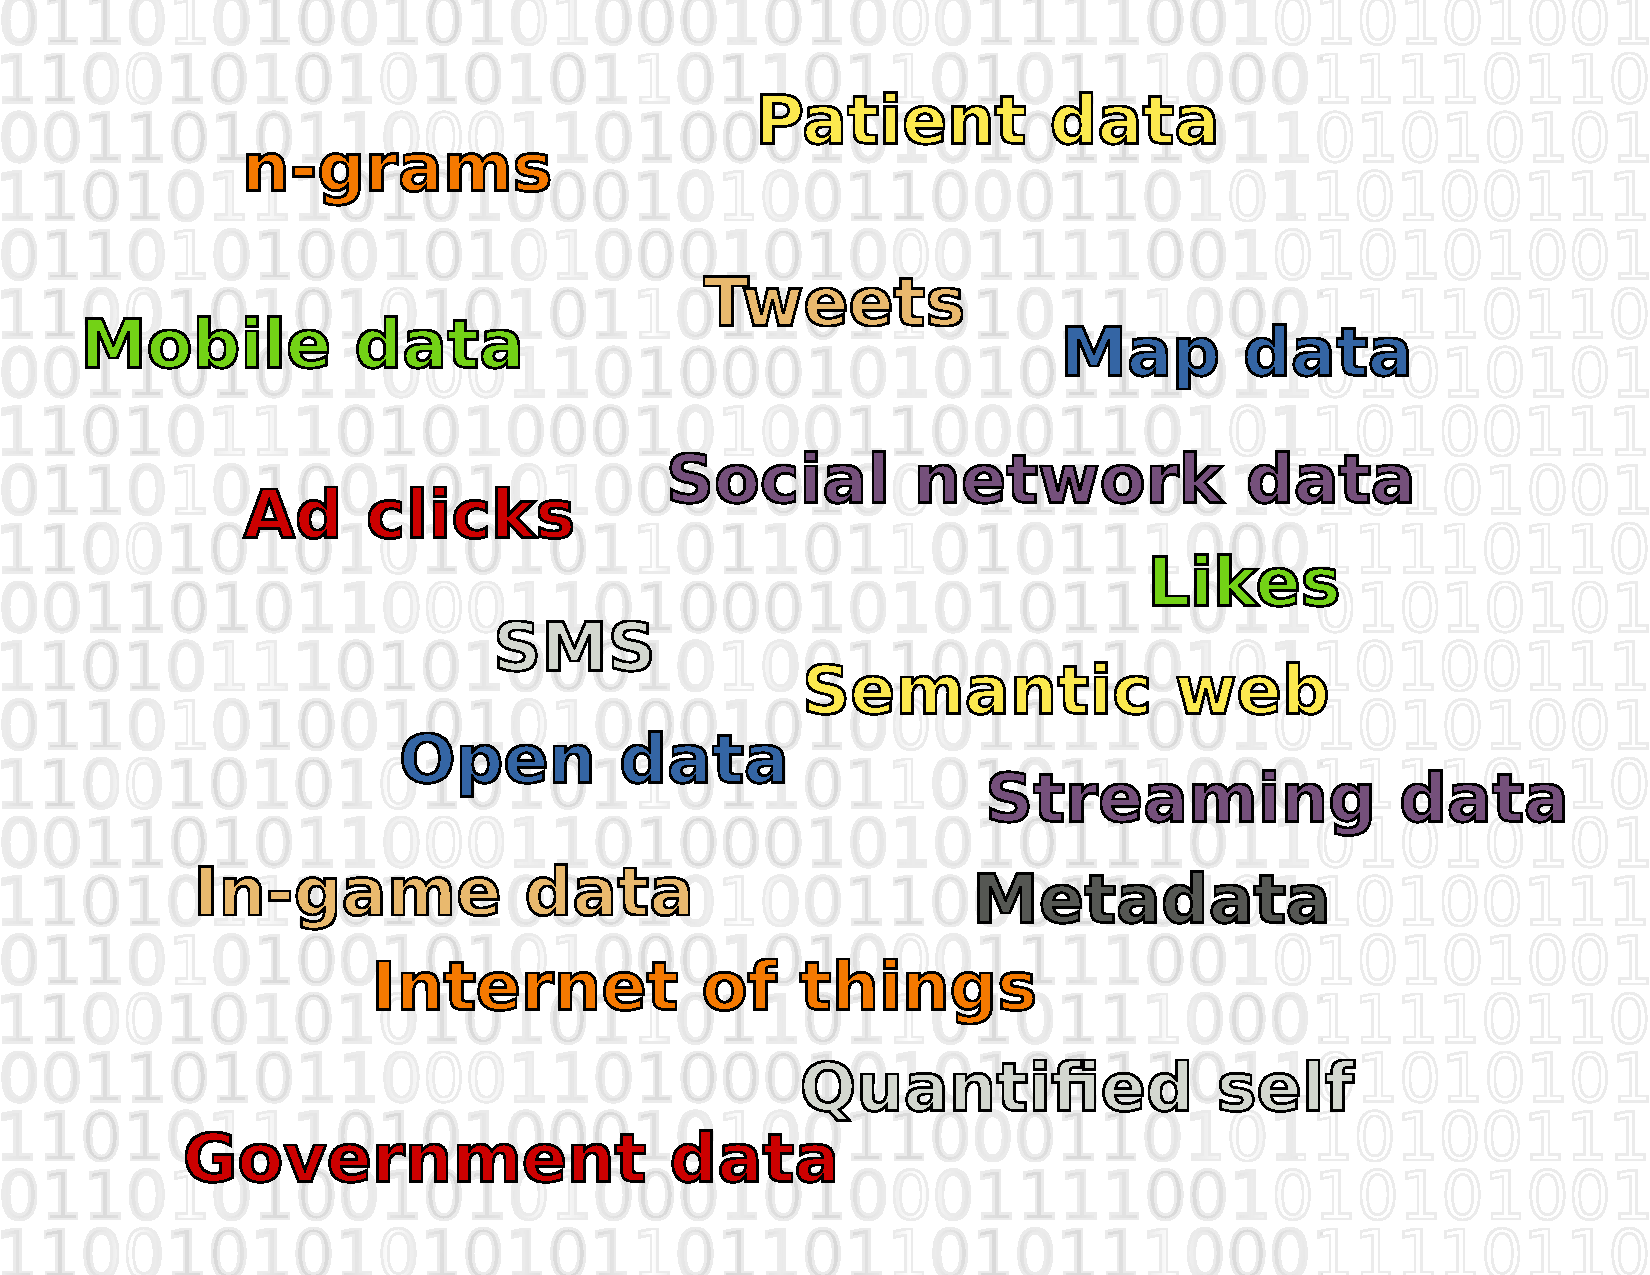
\includegraphics[width=1\textwidth]{graphics/data_cloud2.pdf}
\end{center}
\end{frame}

%%%%%%%%%%%%%%%%%%%%%%%%%%%%%%%%%%%%%%%%%%%%%%%%%%%%%%%%%%%%%%%%%%%%%%%%%%%%%%%%%%%%%%%%%%%%%%%%%

\begin{frame}
%\frametitle{Suddenly data is everywhere!}
\begin{center}

\includegraphics[width=1\textwidth]{graphics/big-data1.pdf}

\bigskip
\bigskip

\begin{itemize}
	\item<2-> How big is big?
	\item<3-> Bigger than a single machine(?)
	\item<4-> What makes it interesting?
\end{itemize}

\end{center}
\end{frame}

%%%%%%%%%%%%%%%%%%%%%%%%%%%%%%%%%%%%%%%%%%%%%%%%%%%%%%%%%%%%%%%%%%%%%%%%%%%%%%%%%%%%%%%%%%%%%%%%%

\begin{frame}
\frametitle{How did we get to ''Big Data''?}

\begin{center}

\begin{columns}

\begin{column}{0.5\textwidth}
\begin{center}
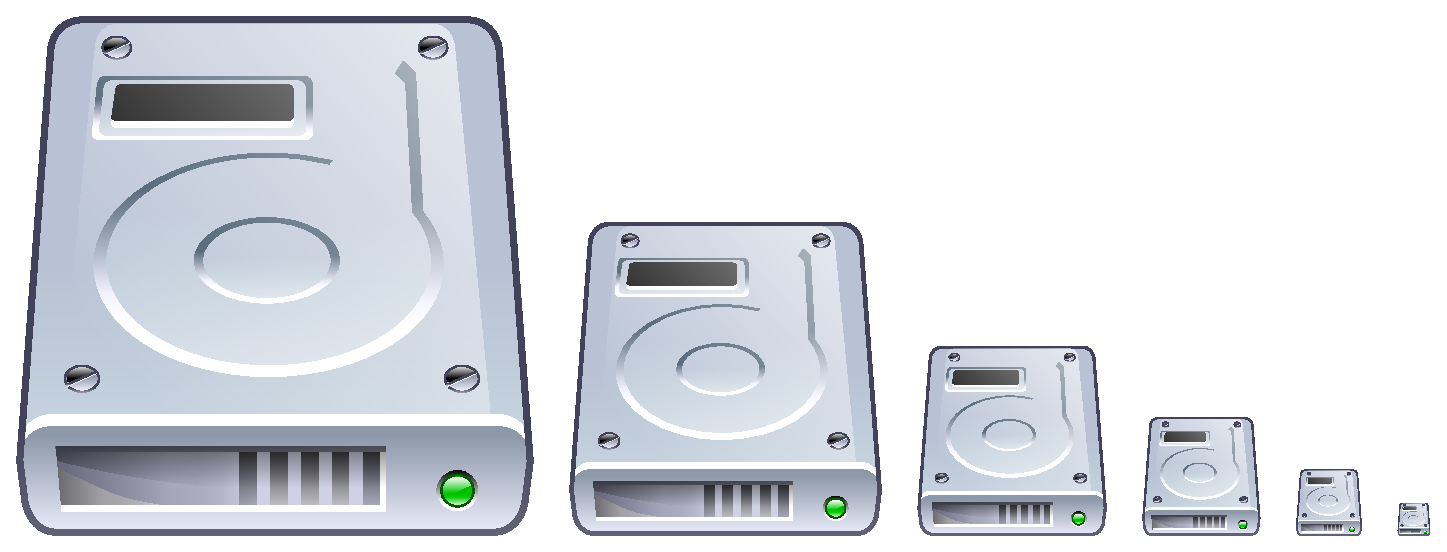
\includegraphics[width=0.5\textwidth]{graphics/hard_drives1.pdf}\\
\bigskip
\bigskip
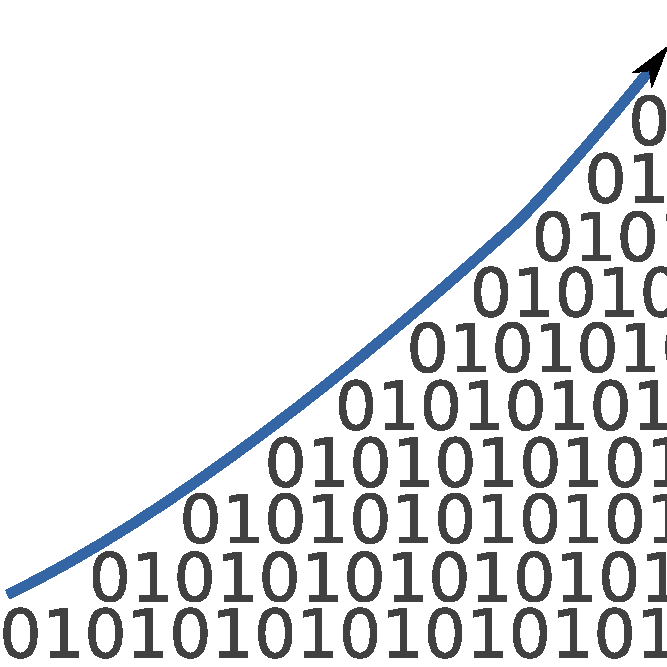
\includegraphics[width=0.3\textwidth]{graphics/data_increase.pdf}\\
\bigskip
\bigskip
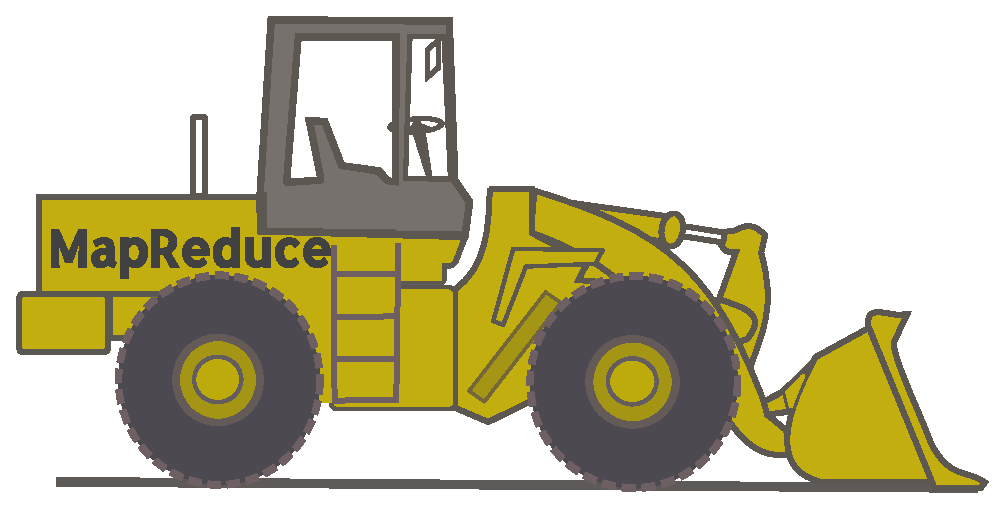
\includegraphics[width=0.6\textwidth]{graphics/Loader.pdf}
\end{center}
\end{column}

\begin{column}{0.5\textwidth}
Exponential drop in storage costs.\\
\begin{itemize}
    \tiny{\item 1GB: 2000 = \$10 $\to$ 2010 = \$0.10}
\end{itemize}
\bigskip
\bigskip


Much more data available.\\
\begin{itemize}
    \tiny{\item Social network and smart phone data}
    \item \tiny{Global internet access up 500\% in past decade}
\end{itemize}
\bigskip
\bigskip
\bigskip

Large scale data processing tools developed.
\end{column}

\end{columns}

\end{center}

\end{frame}

%%%%%%%%%%%%%%%%%%%%%%%%%%%%%%%%%%%%%%%%%%%%%%%%%%%%%%%%%%%%%%%%%%%%%%%%%%%%%%%%%%%%%%%%%%%%%%%%

\begin{frame}
\frametitle{MapReduce, Hadoop, and friends}
\begin{center}
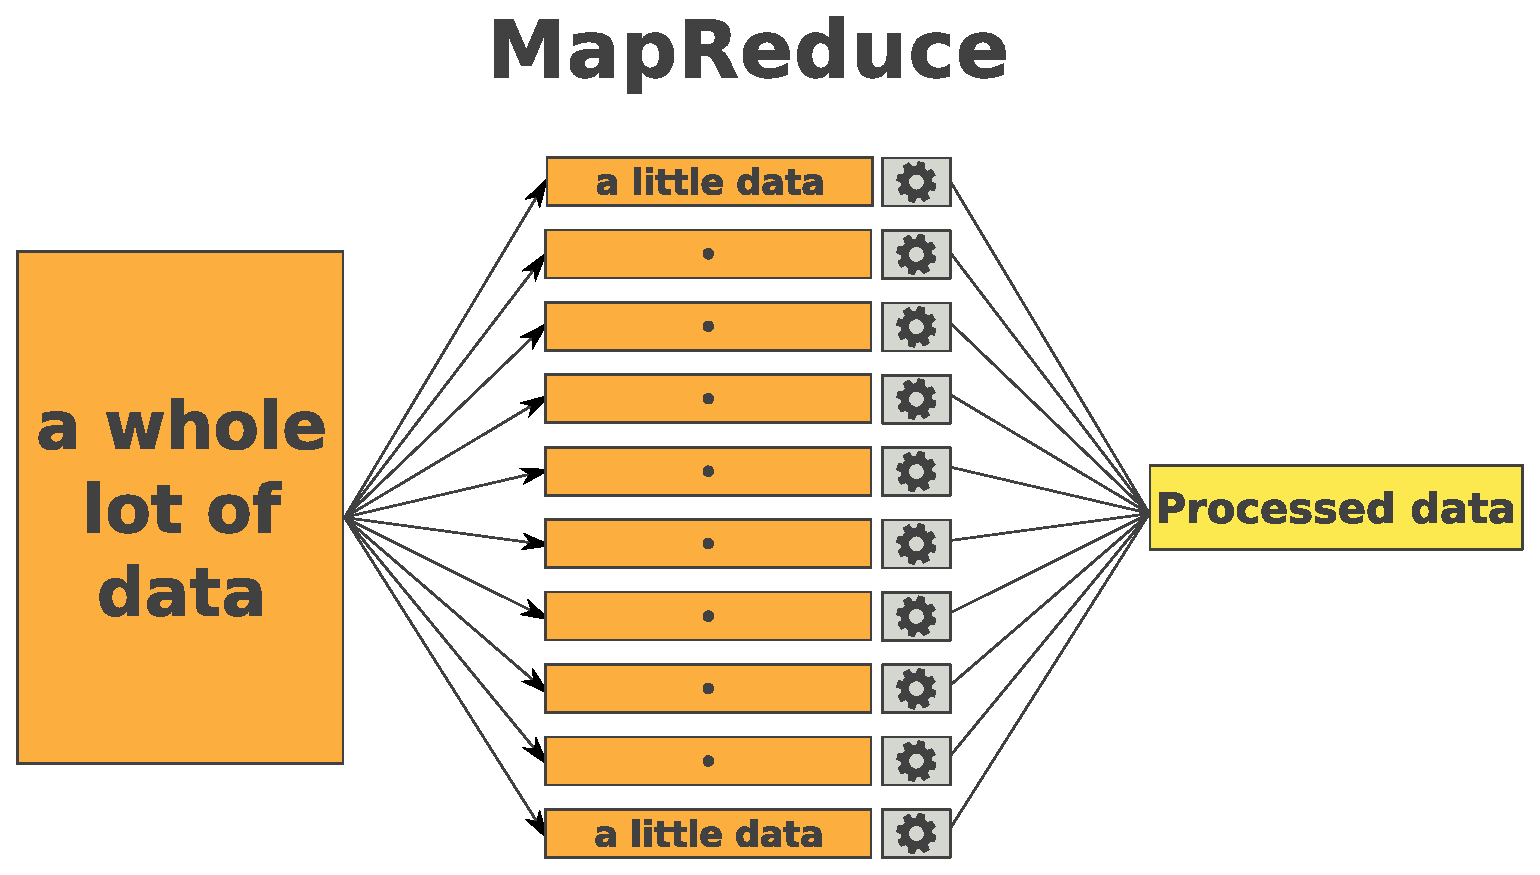
\includegraphics[width=0.7\textwidth]{graphics/mapreduce.pdf}

\pause

\begin{block}{Hadoop}
\begin{itemize}
	\item Open source implementation of MapReduce from Yahoo (2005).
	\item Hadoop + commercial cloud = big data processing.
	\item Basis for an ecosystem of tools.
\end{itemize}
\end{block}
\end{center}
\end{frame}

%%%%%%%%%%%%%%%%%%%%%%%%%%%%%%%%%%%%%%%%%%%%%%%%%%%%%%%%%%%%%%%%%%%%%%%%%%%%%%%%%%%%%%%%%%%%%%%%%

\begin{frame}
\frametitle{(Big) Data in action}
\framesubtitle{Recommendations}
\begin{center}

\begin{columns}

\begin{column}{0.3\textwidth}

\includegraphics[width=1\textwidth]{graphics/Netflix_logo.pdf}
\end{column}

\begin{column}{0.65\textwidth}
\begin{itemize}
\item Recommends ``similar'' movies.
\item Uses customer ratings to infer statistical connections.
\item Algorithms scale much better than humans.
\end{itemize}
\end{column}

\end{columns}

\bigskip
\bigskip

\begin{exampleblock}{Other product recommendation systems}
\begin{itemize}
	\item Retail: Amazon
	\item Radio: Last.fm, Pandora, Spotify
	\item Apps: iTunes, Google Play
\end{itemize}
\end{exampleblock}

\end{center}
\end{frame}

%%%%%%%%%%%%%%%%%%%%%%%%%%%%%%%%%%%%%%%%%%%%%%%%%%%%%%%%%%%%%%%%%%%%%%%%%%%%%%%%%%%%%%%%%%%%%%%%%

\begin{frame}
\frametitle{(Big) Data in action}
\framesubtitle{You might know}
\begin{center}


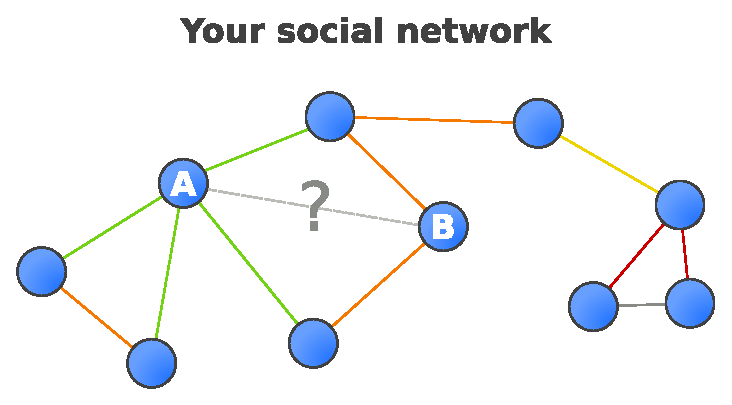
\includegraphics[width=1\textwidth]{graphics/Social-network.pdf}

\bigskip

\begin{itemize}
	\item As seen on LinkedIn, Facebook, Google+, Twitter, etc.
\end{itemize}

\end{center}
\end{frame}

%%%%%%%%%%%%%%%%%%%%%%%%%%%%%%%%%%%%%%%%%%%%%%%%%%%%%%%%%%%%%%%%%%%%%%%%%%%%%%%%%%%%%%%%%%%%%%%%%

\begin{frame}
\frametitle{Data Science}

\begin{center}

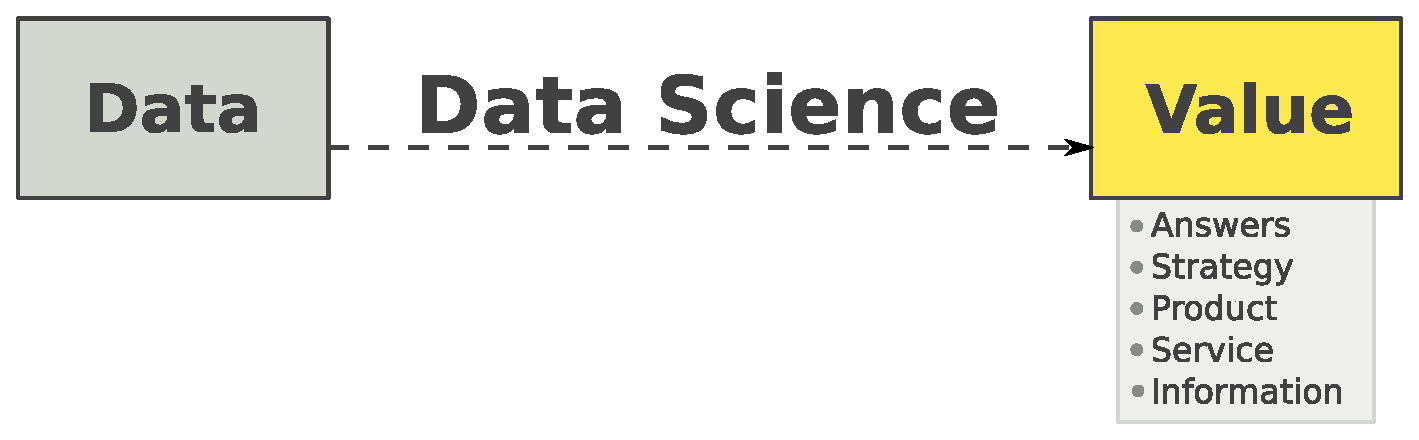
\includegraphics[width=1\textwidth]{graphics/value.pdf}

\bigskip

\begin{itemize}
	\item<1-> Data science is the process of extracting value from data.
	\item<2-> Data science is a buzz word.
\end{itemize}

\end{center}

\end{frame}

%%%%%%%%%%%%%%%%%%%%%%%%%%%%%%%%%%%%%%%%%%%%%%%%%%%%%%%%%%%%%%%%%%%%%%%%%%%%%%%%%%%%%%%%%%%%%%%%%

\begin{frame}
\frametitle{Data Science}

\begin{center}

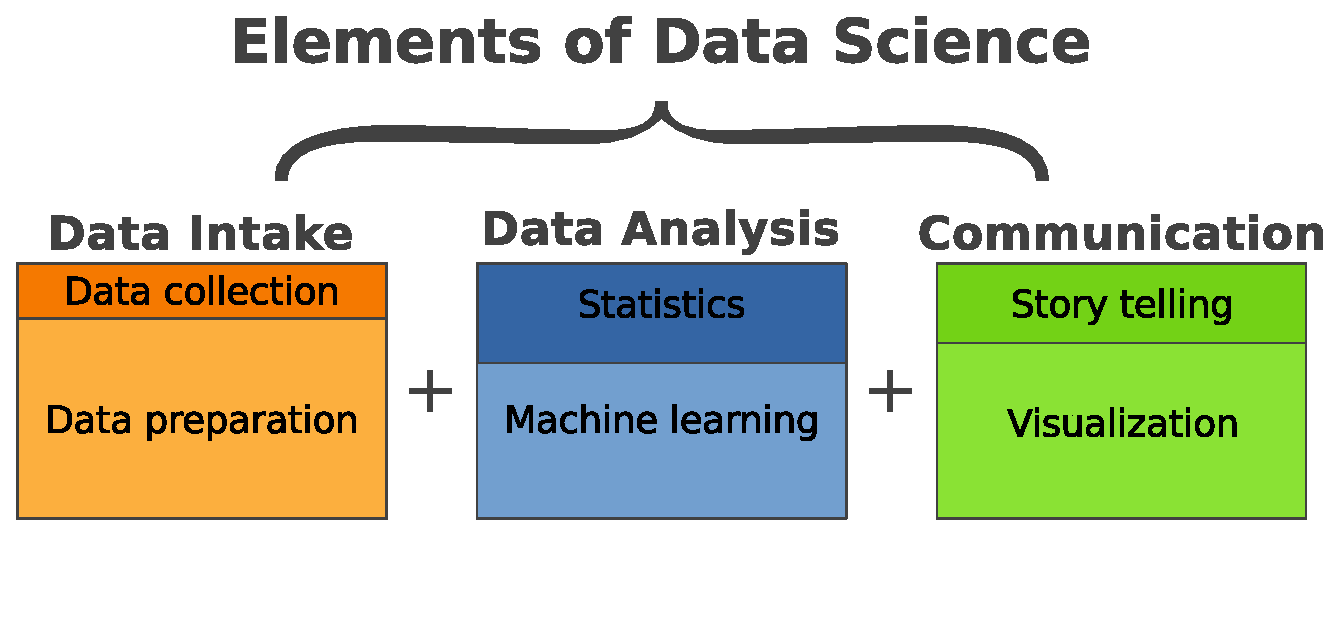
\includegraphics[width=1\textwidth]{graphics/components.pdf}


\end{center}

\end{frame}

%%%%%%%%%%%%%%%%%%%%%%%%%%%%%%%%%%%%%%%%%%%%%%%%%%%%%%%%%%%%%%%%%%%%%%%%%%%%%%%%%%%%%%%%%%%%%%%%%

\begin{frame}
\frametitle{Data Science}
\setcounter{framenumber}{9}
\begin{center}

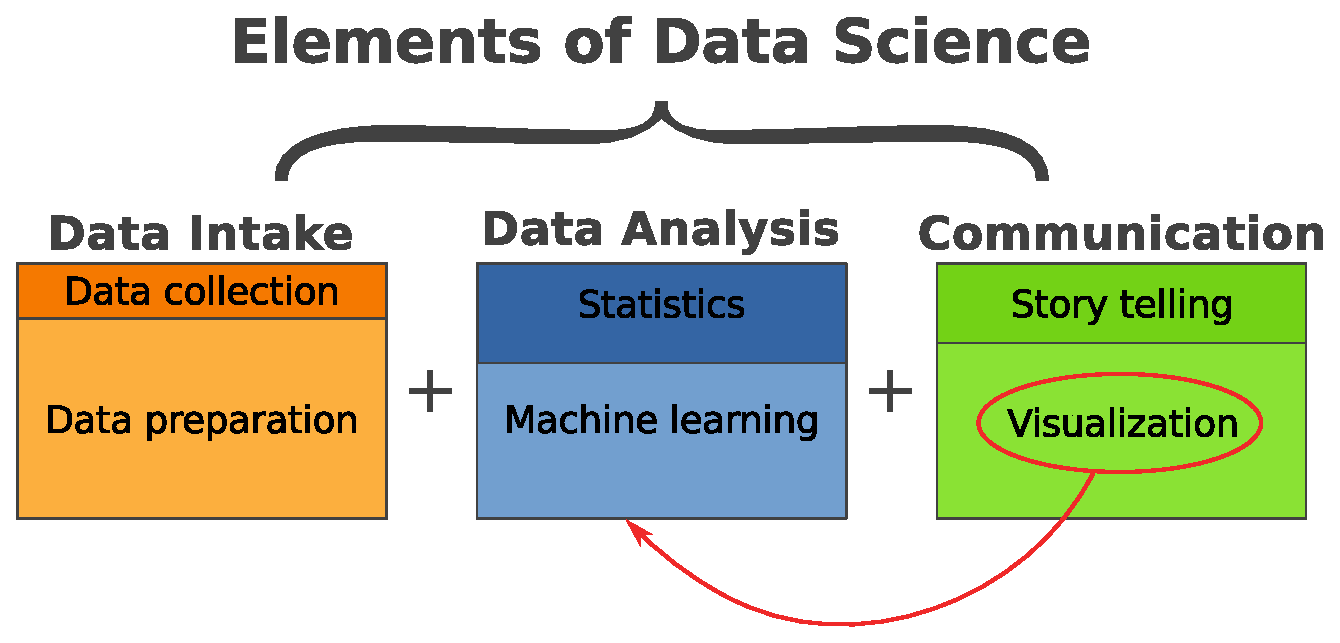
\includegraphics[width=1\textwidth]{graphics/components-b.pdf}


\end{center}

\end{frame}

%%%%%%%%%%%%%%%%%%%%%%%%%%%%%%%%%%%%%%%%%%%%%%%%%%%%%%%%%%%%%%%%%%%%%%%%%%%%%%%%%%%%%%%%%%%%%%%%%
\begin{frame}
\frametitle{Data collection and preparation}
\begin{center}


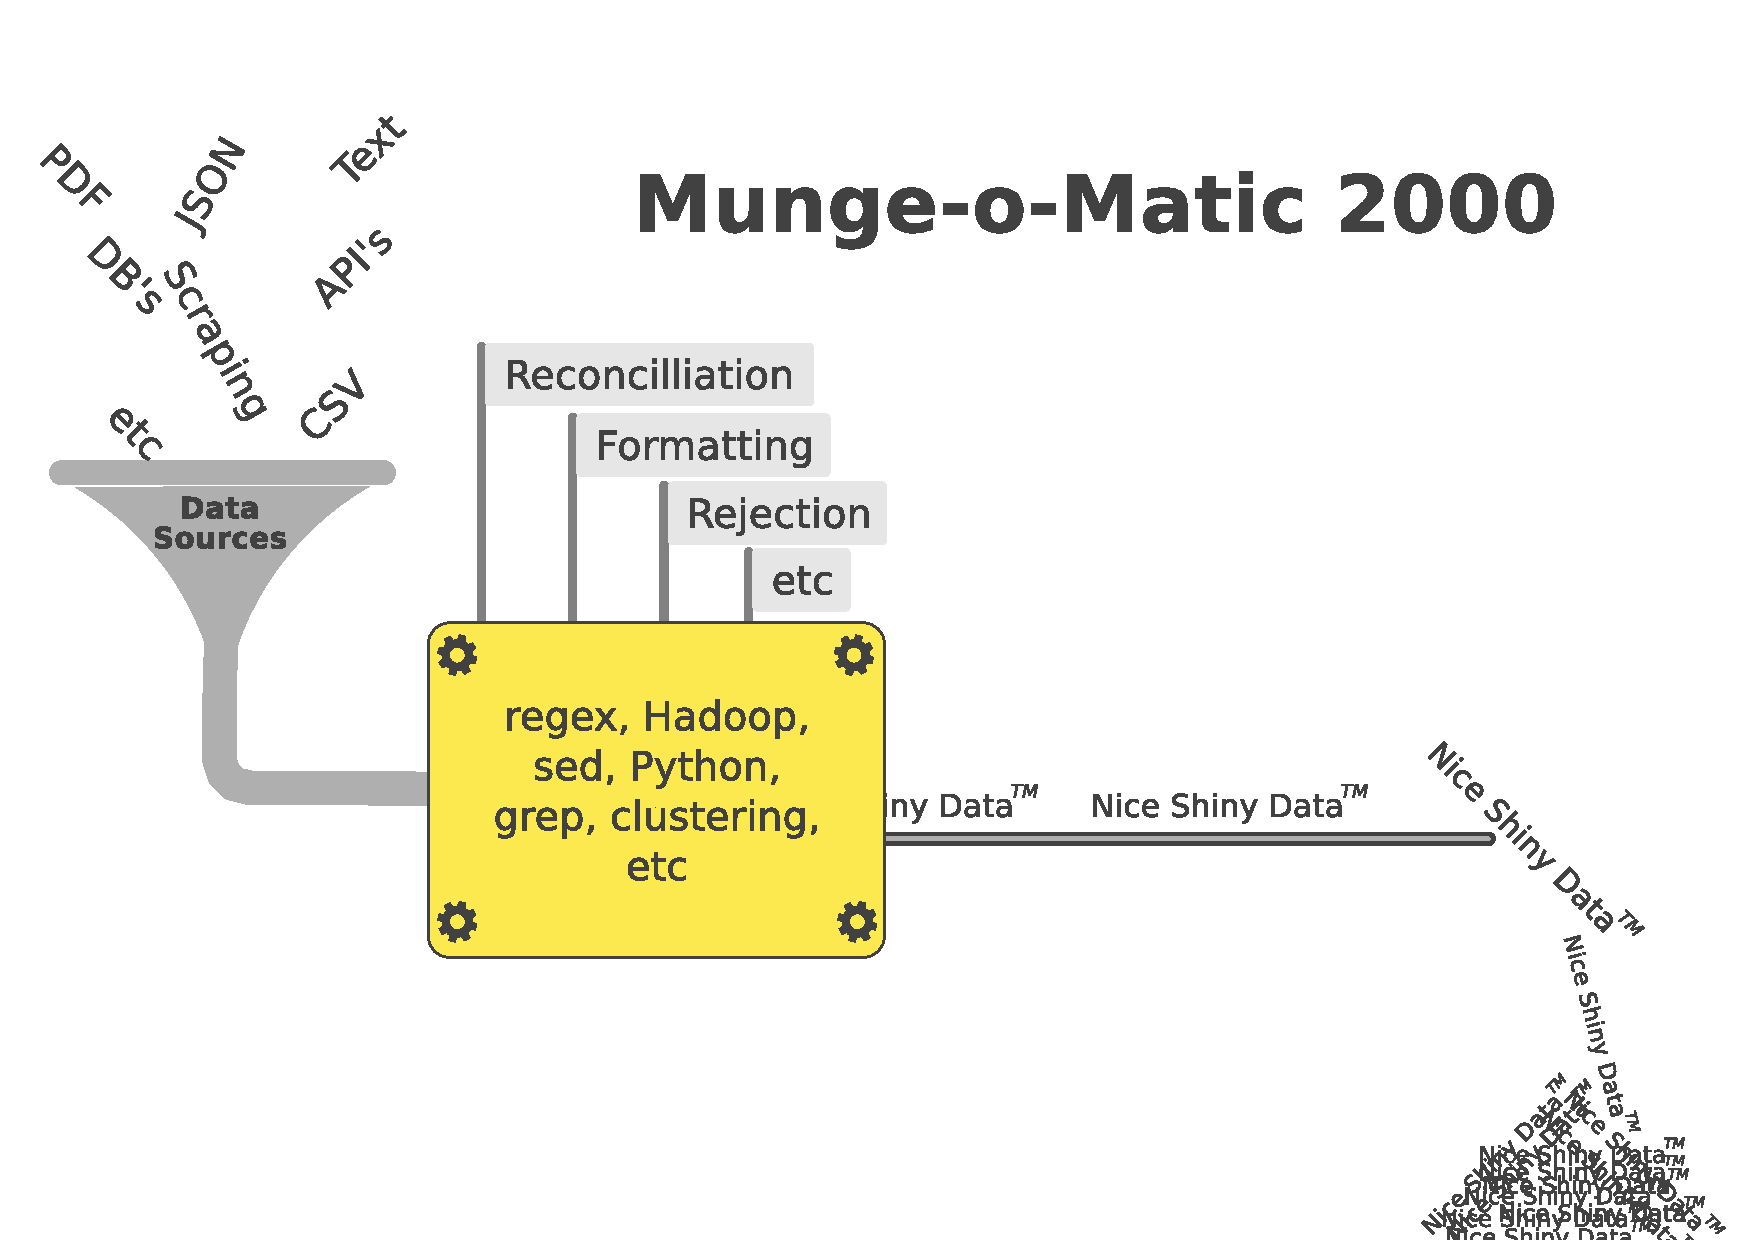
\includegraphics[width=0.9\textwidth]{graphics/data_preparation.pdf}

\end{center}
\end{frame}

%%%%%%%%%%%%%%%%%%%%%%%%%%%%%%%%%%%%%%%%%%%%%%%%%%%%%%%%%%%%%%%%%%%%%%%%%%%%%%%%%%%%%%%%%%%%%%%%%

\begin{frame}
\frametitle{Statistics}

\begin{center}
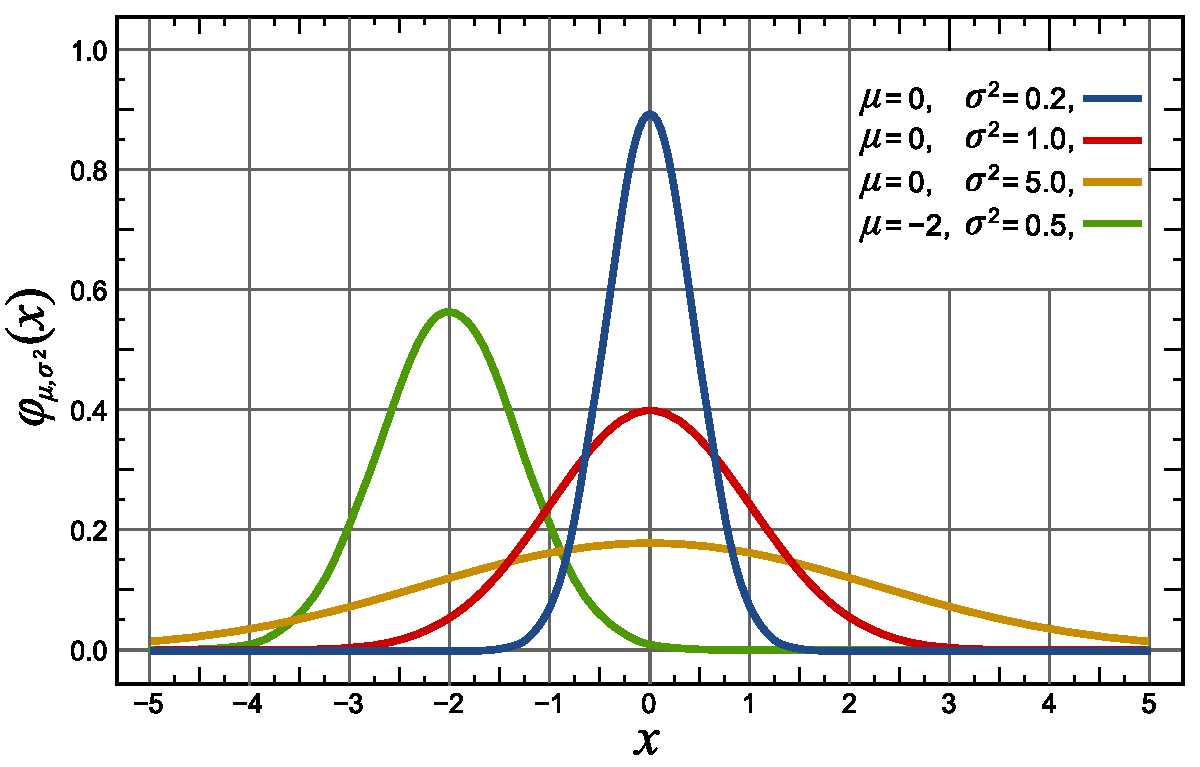
\includegraphics[width=0.5\textwidth]{graphics/Normal_Distribution_PDF.pdf}

\begin{columns}

\begin{column}{0.5\textwidth}
\begin{center}
\begin{itemize}
\item Traditional statistics heavily employed.
\item Hypothesis testing.
\item Experimental design.
\end{itemize}
\end{center}
\end{column}

\begin{column}{0.5\textwidth}
\begin{itemize}
\item Regression analysis.
\item Statistical modeling.
\item Bayesian statistics.
\end{itemize}
\end{column}

\end{columns}

\end{center}

\end{frame}

%%%%%%%%%%%%%%%%%%%%%%%%%%%%%%%%%%%%%%%%%%%%%%%%%%%%%%%%%%%%%%%%%%%%%%%%%%%%%%%%%%%%%%%%%%%%%%%%%

\begin{frame}
\frametitle{Machine Learning}

\begin{center}
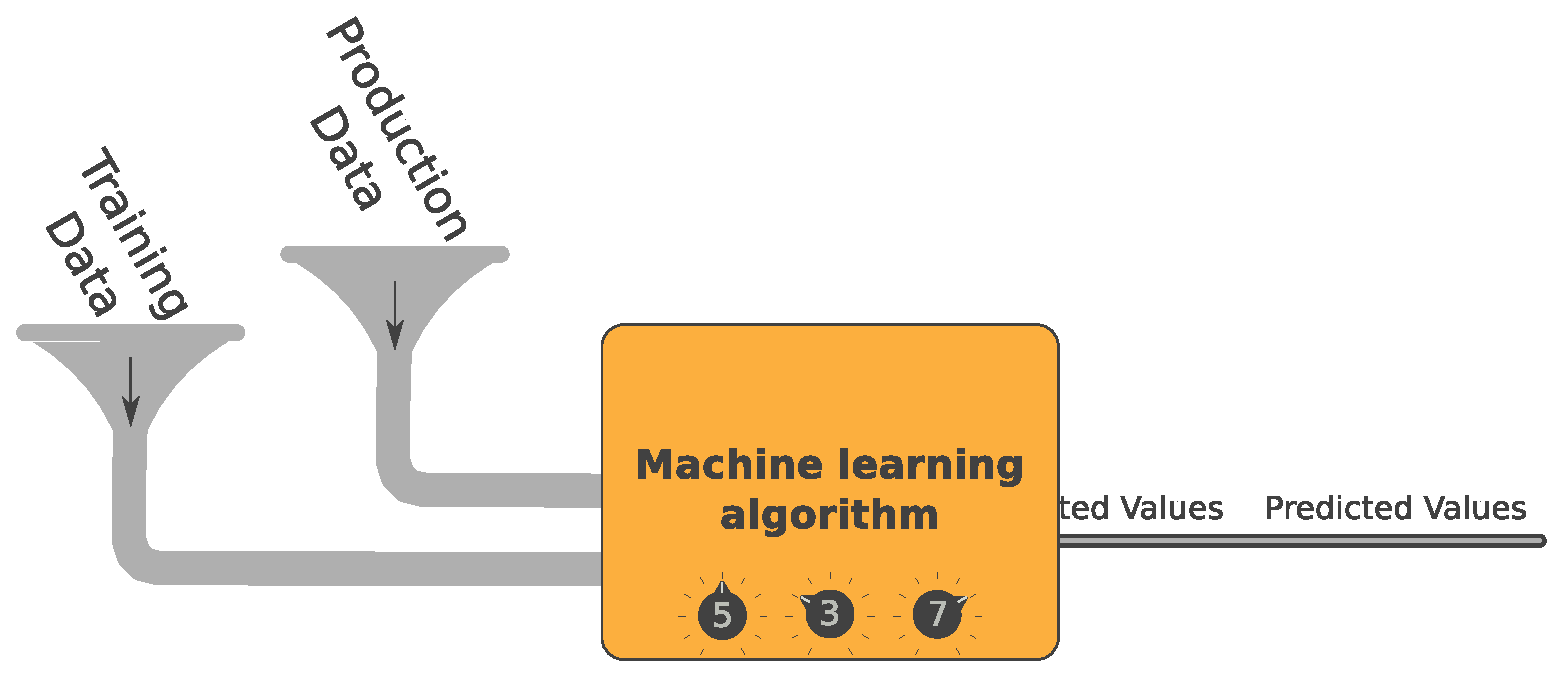
\includegraphics[width=1.0\textwidth]{graphics/machine_learning.pdf}

\begin{columns}

\begin{column}{0.5\textwidth}
\begin{center}
\begin{itemize}
\item Value prediction via AI.
	\begin{itemize}
	\tiny{\item Regression, categorization, clustering.}
	\end{itemize}
\item Random forests, support vector machines, neural networks, etc.
\end{itemize}
\end{center}
\end{column}

\begin{column}{0.5\textwidth}
\begin{itemize} 
\item More training data = better.
\item Less concerned with explanatory power.
\end{itemize}
\end{column}

\end{columns}

\end{center}

\end{frame}

%%%%%%%%%%%%%%%%%%%%%%%%%%%%%%%%%%%%%%%%%%%%%%%%%%%%%%%%%%%%%%%%%%%%%%%%%%%%%%%%%%%%%%%%%%%%%%%%%

\begin{frame}
\frametitle{Story Telling}

\begin{center}


\begin{columns}

\begin{column}{0.5\textwidth}
\begin{center}
\begin{itemize}
\item Presenting results in an audience-appropriate and understandable way.
\item Providing results and clear limitations on those results.
\end{itemize}
\end{center}
\end{column}

\begin{column}{0.5\textwidth}
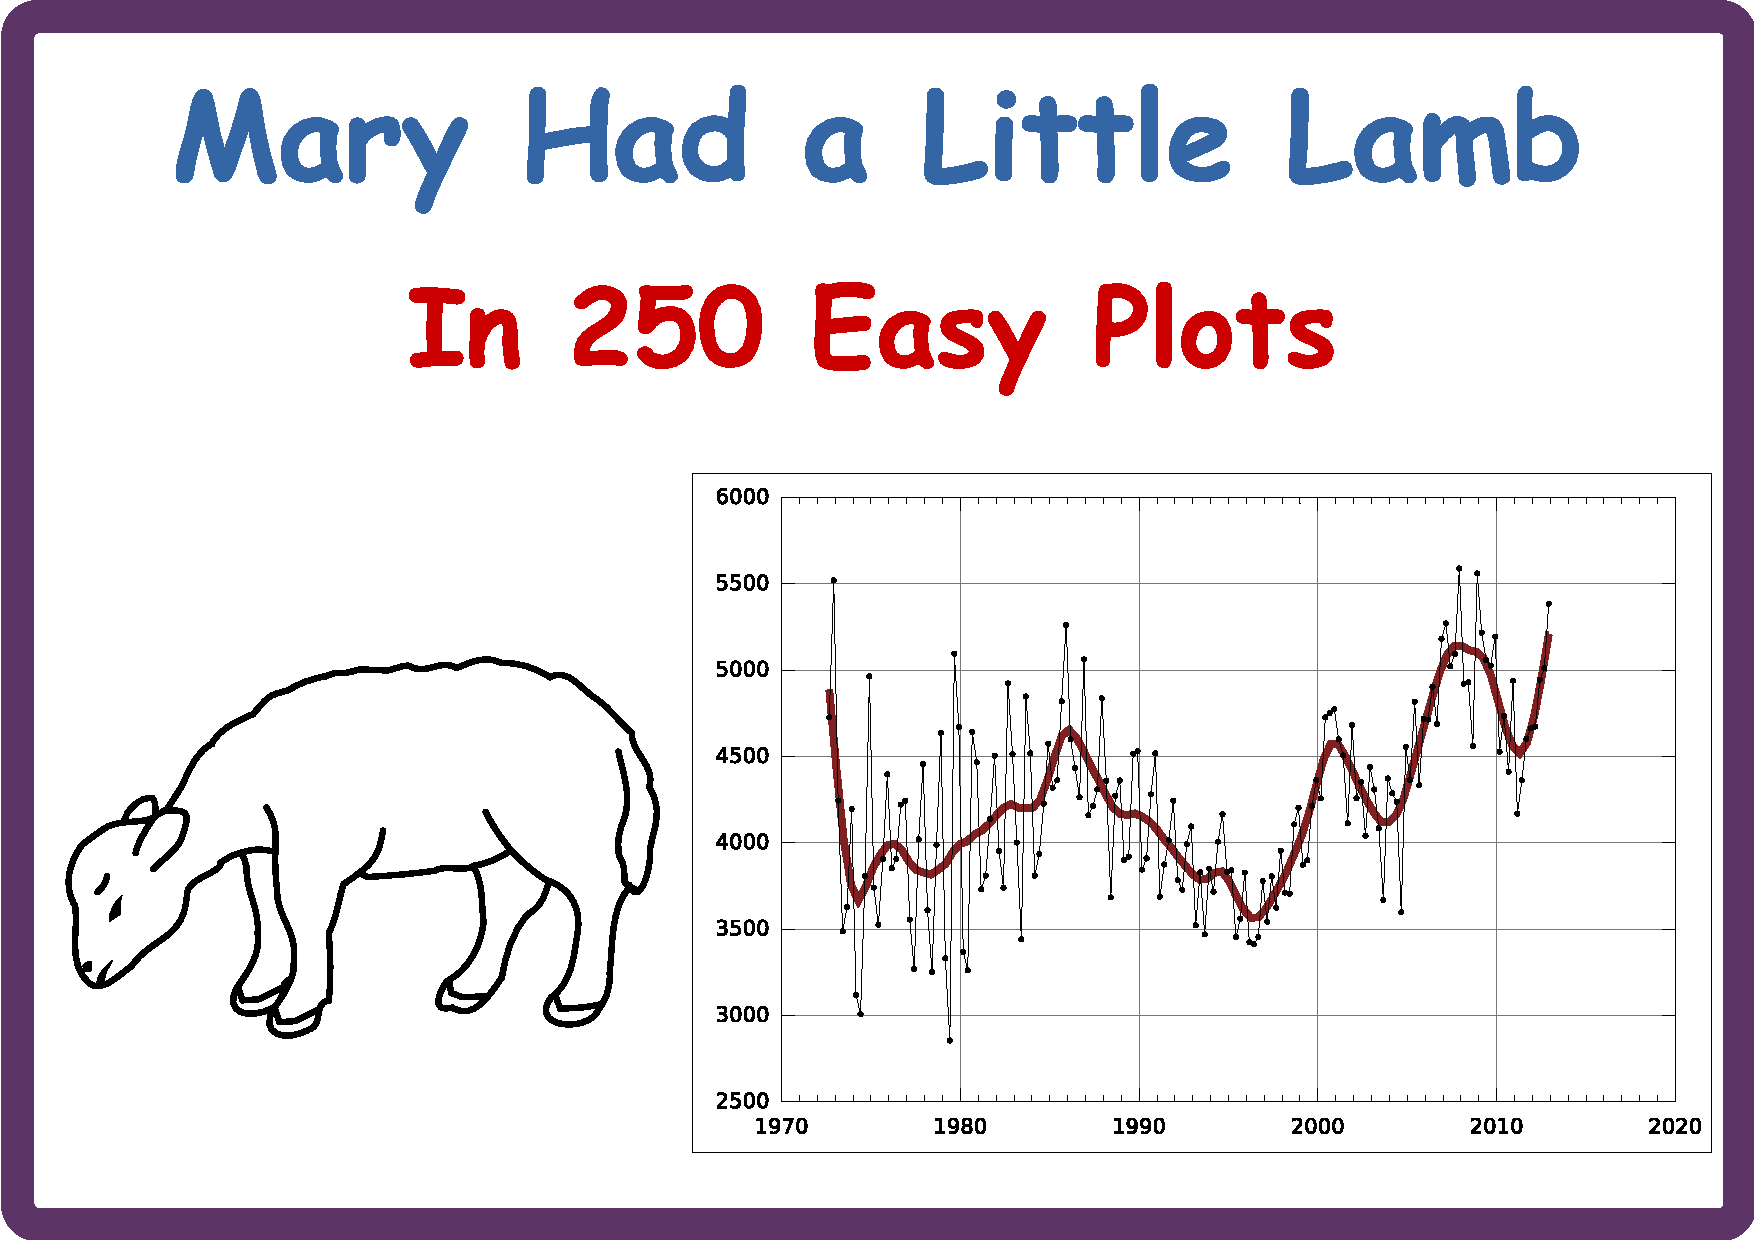
\includegraphics[width=1.0\textwidth]{graphics/mary_had.pdf}
\end{column}

\end{columns}

\end{center}

\end{frame}

%%%%%%%%%%%%%%%%%%%%%%%%%%%%%%%%%%%%%%%%%%%%%%%%%%%%%%%%%%%%%%%%%%%%%%%%%%%%%%%%%%%%%%%%%%%%%%%%%
